\documentclass[11pt]{article}

\usepackage[a4paper,margin=1in]{geometry}
\usepackage[T1]{fontenc}
\usepackage{lmodern}
\usepackage{microtype}
\usepackage{amsmath,amssymb}
\usepackage{graphicx}
\usepackage{booktabs}
\usepackage{caption}
\usepackage{subcaption}
\usepackage{xcolor}
\usepackage[numbers,sort&compress]{natbib}
\usepackage[colorlinks=true,linkcolor=black,citecolor=blue!50!black,urlcolor=blue!50!black]{hyperref}
\usepackage{siunitx}

\newcommand{\iscap}{\textsc{is-capitalized}}
\newcommand{\code}[1]{\texttt{#1}}

\title{\bfseries Does the Standard Sparse-Autoencoder \\ Feature-Absorption Metric Over-Report for Non-Spelling Features?\\[2pt]
\large A Cross-Metric, Cross-Model Study}

\author{Jakub Dvo\v{r}\'ak\\
\normalsize Faculty of Mathematics and Physics, Charles University, Prague\\
\normalsize \texttt{absorption-atlas} technical report}

\date{July 2026}

\begin{document}
\maketitle

\begin{abstract}
\noindent
Sparse autoencoders (SAEs) are meant to decompose language-model activations into monosemantic
features, but \emph{feature absorption}---where a general feature silently fails on some tokens while a
token-specific latent carries the concept---undermines that promise. Absorption is quantified in the
literature almost exclusively on a single task, ``does this token start with letter $X$,'' and with two
different metrics: an older \emph{ablation} (behavioral) metric and the current SAEBench-standard
\emph{projection} (representational) metric. We ask whether the two metrics agree once absorption is
measured on a structurally different, non-spelling property. Running both metrics on
\iscap{} across Gemma-2-2b and Gemma-2-9b (Gemma Scope $16$k SAEs), we find that they
\emph{disagree}: the projection metric reports single-dominant-latent absorption modestly above its
random-direction null ($0.14$, $95\%$ CI $[0.085,0.200]$ vs.\ $0.04$; $n{=}130$---marginal), whereas the
ablation metric reports exactly zero on $273/273$ candidate tokens, on \emph{both} models. Two controls
rule out the mundane explanations: it is not task performance (Gemma-2-9b performs \iscap{} at $0.91$
accuracy, yet ablation stays $0.0$) and not a dead layer (at the same layer, spelling ablation fires at
$0.045$; at matched task accuracy it fires at ${\sim}0.026$ for spelling while \iscap{} remains $0.0$).
We conclude that the field-standard projection absorption metric appears to over-report single-latent
absorption for a distributed structural feature that has no causal correlate. As a secondary result, we
show that ablation-based absorption is itself task-accuracy-sensitive within the spelling task. We
reproduce the known first-letter absorption and its L0 dependence as pipeline validation. Effects are
near-floor and the study spans one property, one model family, and one SAE recipe; we treat the result as
a metric-validity caveat and an argument that representational absorption signals require causal
validation.
\end{abstract}

\section{Introduction}
Sparse autoencoders (SAEs) have become a leading tool for decomposing the internal activations of
language models into a large, sparse set of features that are, ideally, monosemantic and human-interpretable
\citep{elhage2022superposition,bricken2023monosemanticity,cunningham2023sparse,templeton2024scaling}. A central threat to this interpretation is
\emph{feature absorption} \citep{chanin2024absorption}: a latent that appears to encode a general concept
(e.g.\ ``starts with the letter S'') silently deactivates on a subset of tokens, while a more specific,
token-aligned latent (e.g.\ a ``short'' latent) absorbs the general direction and carries the concept for
those tokens. Absorption means the ``general'' feature is not what it seems, which is corrosive for any
downstream use of SAE features as reliable concept detectors.

Despite its importance, absorption has been measured almost exclusively on one family of tasks:
first-letter (and, in benchmarks, first-letter only) spelling, where ground truth is trivially available
\citep{chanin2024absorption,karvonen2025saebench}. Chanin et al.\ explicitly list ``examples of feature
absorption unrelated to character identification'' as open future work. Moreover, two distinct metrics are
in use: (i) an \emph{ablation} (behavioral) metric that attributes the model's task answer to individual
SAE latents via integrated gradients \citep{chanin2024absorption}, and (ii) a \emph{projection}
(representational) metric that decomposes the residual stream's projection onto a concept probe direction
into per-latent contributions. The projection metric is the current standard adopted by SAEBench
\citep{karvonen2025saebench}, specifically because the ablation effect decays toward zero in later layers.

This raises a simple, previously untested question: \textbf{do the two absorption metrics agree once we
move off the spelling task?} We answer it for structural, non-spelling token properties---primarily
\iscap{} (whether a token begins with an uppercase letter)---and find that they do not.

\paragraph{Contributions.}
\begin{enumerate}\itemsep2pt
  \item We run \emph{both} standard absorption metrics (projection and ablation) on structural token
  properties, contrasting them directly. To our knowledge this specific comparison has not been reported.
  (We do \emph{not} claim the first measurement on non-character properties: \citet{chanin2025hedging}
  already probe part-of-speech with $k$-sparse probing.)
  \item We report a \emph{metric disagreement}: for \iscap{}, projection reports above-null absorption
  while ablation reports a clean zero, with bootstrap confidence intervals.
  \item We isolate the cause with two controls---a cross-model task-ability control (Gemma-2-9b) and a
  layer-/accuracy-matched spelling control---ruling out both ``the model cannot do the task'' and ``the
  layer is dead.'' The residual explanation is a genuine property-level difference in absorption structure.
  \item As a secondary, controlled result, we show the ablation metric is itself sensitive to task accuracy
  within the spelling task, whereas the projection metric is not.
\end{enumerate}

\section{Background and Related Work}
\paragraph{Sparse autoencoders and monosemanticity.}
An SAE reconstructs a model activation $\mathbf{x}\in\mathbb{R}^{d}$ as $\hat{\mathbf{x}}=W_{\mathrm{dec}}
\,\mathbf{a} + \mathbf{b}$ with sparse codes $\mathbf{a}=\mathrm{enc}(\mathbf{x})\ge 0$, trained to trade
off reconstruction against sparsity \citep{bricken2023monosemanticity,cunningham2023sparse}. We use Gemma Scope
\citep{lieberum2024gemmascope}, the open suite of JumpReLU SAEs trained on Gemma-2 \citep{gemmateam2024gemma2}.

\paragraph{Feature absorption and its two metrics.}
\citet{chanin2024absorption} define absorption and measure it on the first-letter task. Their metric is
causal: on a token where the general (``main'') latent is silent, they use integrated-gradient
attribution to check whether a single latent, aligned with a linear probe for the concept, most strongly
supports the model's answer. SAEBench \citep{karvonen2025saebench} standardizes a \emph{projection}
variant---decomposing the residual's projection onto the probe direction into per-latent contributions---
noting that the ablation signal ``goes to zero in later layers.'' Thus the ablation metric is effectively
deprecated in favor of projection; a corollary is that ``ablation reads $0$'' is, in later layers, a known
artifact rather than evidence of no absorption. Our contribution rests precisely on distinguishing that
artifact from a genuine zero via layer- and accuracy-matched controls.

\paragraph{Related mechanisms and mitigations.}
\citet{chanin2025hedging} describe \emph{feature hedging}, whereby narrow SAEs merge correlated features
into distributed, partly-polysemantic latents, and already probe part-of-speech. Hedging is the most
likely mundane mechanism for a structural concept being ``represented but distributed,'' and we engage it
in the discussion. Matryoshka SAEs \citep{bussmann2025matryoshka} are an architecture proposed to reduce
absorption. Separately, \citet{kantamneni2025saeprobing} find SAE latents do not beat raw-activation probing
baselines, situating our missing downstream ``so what'' in a broader debate about SAE utility.

\section{Methods}
\paragraph{Models and SAEs.}
We use Gemma-2-2b (residual stream, layer $12$) and Gemma-2-9b (layer $20$), each with the Gemma Scope
JumpReLU residual SAE of width $16$k, at an average $L0$ near $70$--$82$. Layers are chosen well below the
depth at which the ablation metric is known to fail. All activations are read at the word-token position
of an in-context prompt.

\paragraph{Token properties.}
The concept is elicited by an in-context task with an objective, tokenizer-derivable label: first-letter
and last-letter (26-way), and the binary structural properties \iscap{}, \textsc{all-caps}, and
suffix-\textsc{-ing}/\textsc{-ed}. Only \iscap{} yields a well-powered candidate pool
($n{=}130$--$273$); the others are underpowered ($n{=}9$--$33$) and reported as anecdotes.

\paragraph{Pipeline.}
For each concept we (i) train a linear probe on the residual stream (the ground-truth concept direction);
(ii) run $k$-sparse probing to identify the concept's ``main'' SAE latent(s) via a feature-splitting F1
criterion; and (iii) collect \emph{candidate false negatives}: tokens where the probe fires but the main
latents do not. Absorption is then quantified on these candidates by two metrics.

\paragraph{Ablation (behavioral) metric.}
Following \citet{chanin2024absorption}, on each candidate we run integrated-gradient attribution of SAE
latents to a logit-difference metric for the task answer; a token counts as absorbed if the main latents
are silent, a single latent is the clear most-causal one, and it is probe-aligned. We report the
absorption rate (absorbed / probe-true-positives), with an additive dominance threshold.

\paragraph{Projection (representational) metric.}
We decompose the residual's projection onto the (unit) probe direction $\hat{\mathbf p}$ into per-latent
contributions $c_i = a_i\,(W_{\mathrm{dec},i}\cdot\hat{\mathbf p})$. On a candidate where the main latents
are silent, absorption is present if one non-main latent dominates: $c_{(1)} \ge R\,c_{(2)}$ for a
scale-free dominance ratio $R$. Crucially we add a \textbf{random-direction null}: the same statistic
computed against random unit directions in place of $\hat{\mathbf p}$, averaged over five draws, to control
for the fact that SAE sparsity makes \emph{any} projection tend to be dominated by one active latent. We
report the \emph{conditioned} rate (fraction of main-silent candidates showing single-dominant absorption)
so that the estimate does not bake in main-latent quality.

\paragraph{Task-accuracy measurement and controls.}
For each (property, model) we measure the model's in-context accuracy on the task. To separate
``ablation reads $0$ because the concept is not causally absorbed'' from the two mundane confounds, we use:
(a) a \textbf{cross-model} control (Gemma-2-9b, which performs \iscap{} far better than 2b); (b) a
\textbf{layer-matched} spelling control (first-letter absorption at the same 9b layer/$L0$); and (c) a
\textbf{matched-accuracy} control, obtained by sweeping first-letter task accuracy through the number of
in-context examples and by corrupting a fraction of in-context answers, so we can compare structural and
spelling absorption at equal task accuracy. All statistics use bootstrap $95\%$ confidence intervals; the
single-class (binary-property) pipeline is a re-implementation of the 26-way one and was independently
review-verified.

\section{Results}

\subsection{Reproduction and the L0 law}
As pipeline validation we reproduce first-letter absorption on current Gemma Scope SAEs and recover the
known dependence on SAE sparsity: absorption rises steeply as $L0$ falls (Figure~\ref{fig:l0},
Table~\ref{tab:l0}), sitting a consistent factor below SAEBench's own JumpReLU numbers, as expected for
the more thoroughly trained Gemma Scope SAEs. Last-letter behaves like first-letter (Figure~\ref{fig:prop}),
confirming that within the spelling family absorption is not specific to the first character.

\begin{figure}[t]
  \centering
  \begin{subfigure}[t]{0.49\textwidth}
    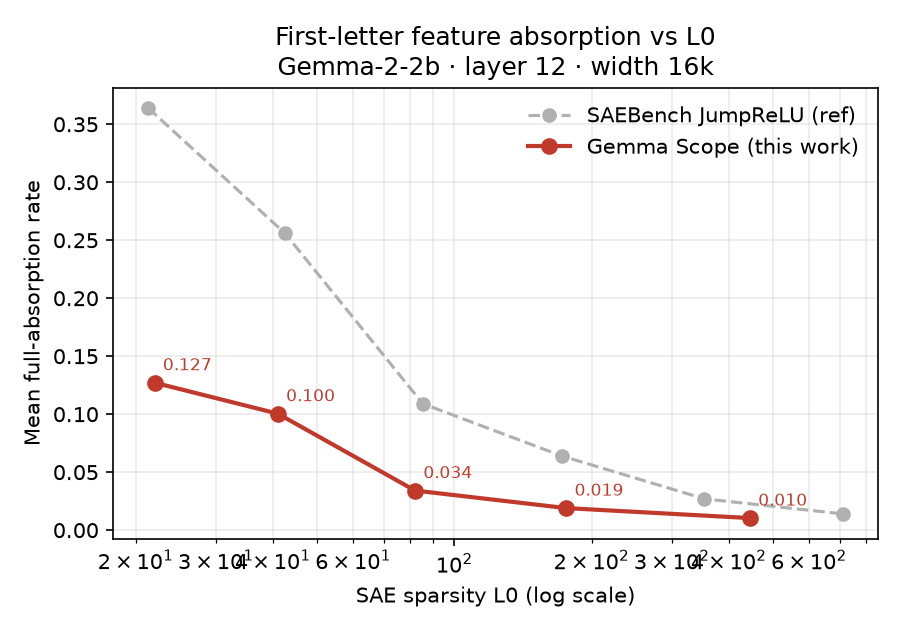
\includegraphics[width=\linewidth]{figures/absorption_vs_l0.png}
    \caption{Absorption vs.\ $L0$ (Gemma Scope vs.\ SAEBench reference).}
    \label{fig:l0}
  \end{subfigure}\hfill
  \begin{subfigure}[t]{0.49\textwidth}
    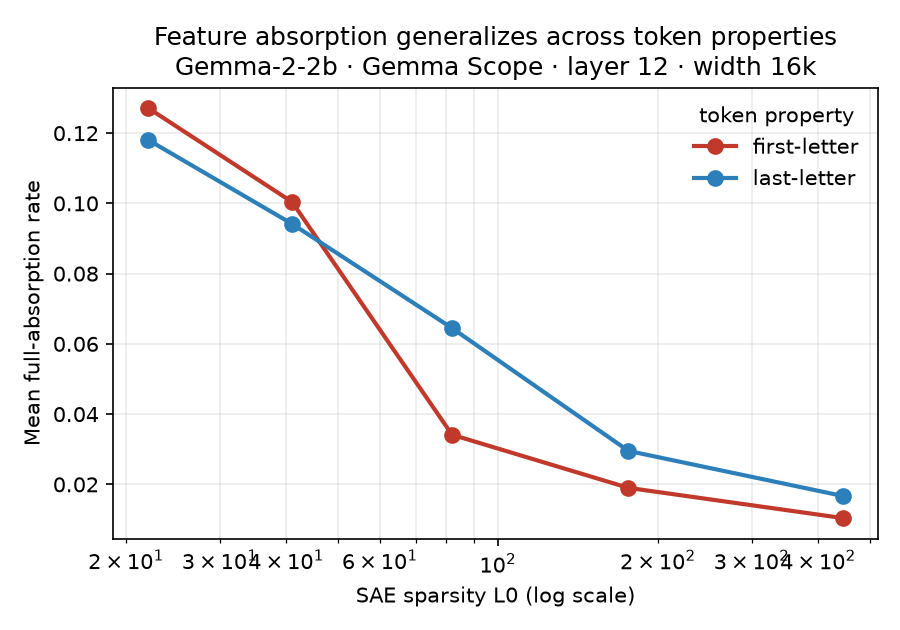
\includegraphics[width=\linewidth]{figures/property_comparison.png}
    \caption{First- vs.\ last-letter absorption vs.\ $L0$.}
    \label{fig:prop}
  \end{subfigure}
  \caption{Reproduction. (a) The first-letter absorption--$L0$ law is recovered on current Gemma Scope SAEs.
  (b) Last-letter tracks first-letter, so within spelling the phenomenon is not first-character-specific.}
\end{figure}

\begin{table}[t]
  \centering
  \caption{Mean absorption rate vs.\ SAE sparsity $L0$ (Gemma-2-2b, layer 12, width 16k). Both spelling
  properties show the expected monotone decrease with $L0$.}
  \label{tab:l0}
  \sisetup{round-mode=places,round-precision=3}
  \begin{tabular}{lccccc}
    \toprule
    $L0$ & 22 & 41 & 82 & 176 & 445 \\
    \midrule
    first-letter & 0.127 & 0.100 & 0.034 & 0.019 & 0.010 \\
    last-letter  & 0.118 & 0.094 & 0.065 & 0.030 & 0.017 \\
    \bottomrule
  \end{tabular}
\end{table}

\subsection{The two metrics disagree on \iscap{}}
Table~\ref{tab:proj} and Figure~\ref{fig:probedir} report the projection metric with its random-direction
null. For spelling, projection absorption is large and far above the null ($0.54$ vs.\ $0.04$ at $R{=}3$).
For \iscap{}, projection absorption is above the null but \emph{marginal} at $n{=}130$ ($0.14$, CI
$[0.085,0.200]$ vs.\ null $0.04$, CI $[0.008,0.077]$), and roughly $4\times$ weaker than spelling.

In sharp contrast, the \emph{ablation} metric reports \iscap{} absorption of exactly $0.0$---on both
Gemma-2-2b and Gemma-2-9b, and on all $273$ candidate tokens of the 9b run (binomial $95\%$ CI
$[0,\,0.011]$). The two metrics thus disagree: projection sees a (weak) absorber; ablation sees none.

\begin{table}[t]
  \centering
  \caption{Projection (representational) single-dominant-latent absorption at dominance $R{=}3$, conditioned
  on the main-latent-silent candidate pool, with bootstrap $95\%$ CIs, vs.\ a random-direction null.}
  \label{tab:proj}
  \begin{tabular}{lccc}
    \toprule
    property & projection [95\% CI] & random null [95\% CI] & $n$ \\
    \midrule
    first-letter & 0.54\ [0.51,\,0.56] & 0.04\ [0.03,\,0.05] & 2085 \\
    \iscap{}     & 0.14\ [0.085,\,0.200] & 0.04\ [0.008,\,0.077] & 130 \\
    \bottomrule
  \end{tabular}
\end{table}

\begin{figure}[t]
  \centering
  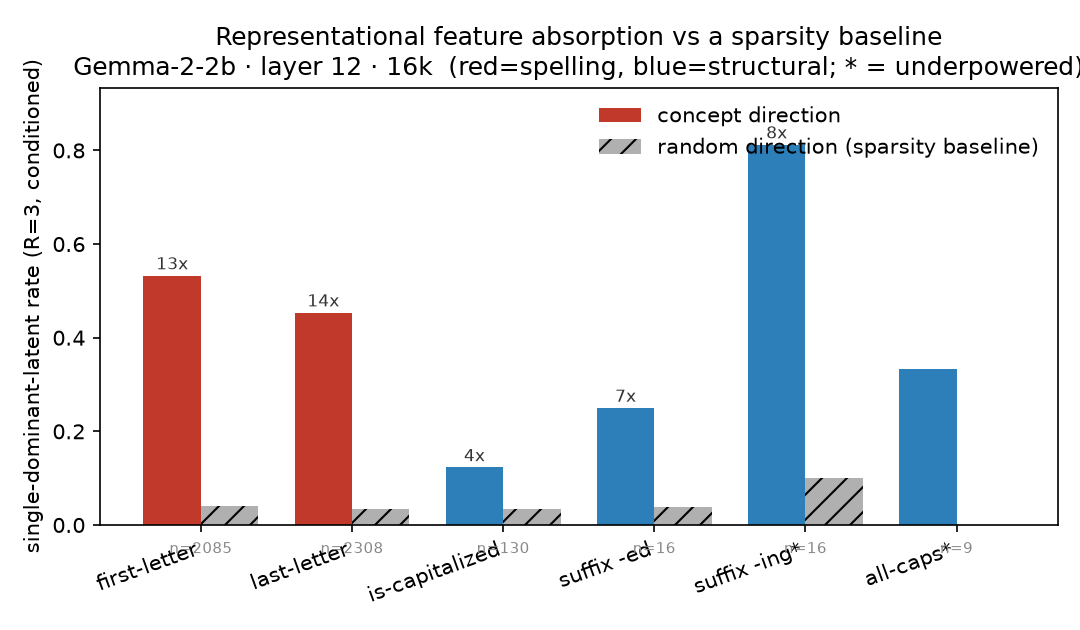
\includegraphics[width=0.62\textwidth]{figures/probedir.png}
  \caption{Projection absorption vs.\ a random-direction sparsity baseline (strict dominance $R{=}3$).
  Spelling (red) is $13$--$14\times$ above the null; structural properties (blue) are above the null but
  much weaker, and \textsc{all-caps}/suffix are underpowered ($\ast$).}
  \label{fig:probedir}
\end{figure}

\subsection{Controls: not task-validity, not a dead layer}
Table~\ref{tab:cross} and Figure~\ref{fig:cross} present the cross-model controls. Because the ablation
metric is known to fail in later layers, the decisive question is whether the \iscap{} zero is genuine.
It is: (i) Gemma-2-9b performs \iscap{} at $0.91$ accuracy---far above 2b's $0.60$---yet ablation absorption
remains $0.0$; and (ii) at the \emph{same} 9b layer/$L0$, first-letter ablation absorption is $0.045$, so
the metric demonstrably fires there. Finally, using the accuracy sweep of \S\ref{sec:mech}, at matched task
accuracy ${\sim}0.9$ first-letter ablation absorption is ${\sim}0.026$ while \iscap{} is $0.0$. The
structural zero is therefore not explained by task ability or layer.

\begin{table}[t]
  \centering
  \caption{Cross-model behavioral (ablation) absorption. Spelling absorbs on both models; \iscap{} on
  neither, even as its task accuracy rises from $0.60$ (2b) to $0.91$ (9b).}
  \label{tab:cross}
  \begin{tabular}{llcc}
    \toprule
    property & model / layer & task accuracy & ablation absorption \\
    \midrule
    first-letter & Gemma-2-2b / L12 & ${\sim}0.95$ & 0.032 \\
    first-letter & Gemma-2-9b / L20 & ${\sim}0.96$ & 0.045 \\
    \iscap{}     & Gemma-2-2b / L12 & 0.60 & 0.000 \\
    \iscap{}     & Gemma-2-9b / L20 & 0.91 & 0.000 \\
    \bottomrule
  \end{tabular}
\end{table}

\begin{figure}[t]
  \centering
  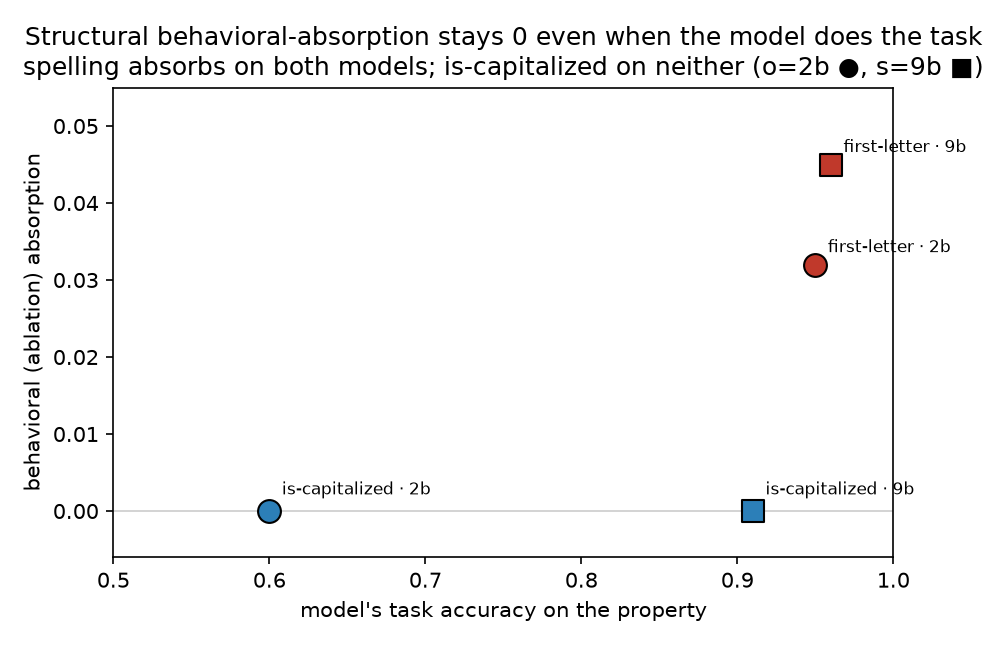
\includegraphics[width=0.62\textwidth]{figures/crossmodel.png}
  \caption{The structural (blue) behavioral-absorption zero persists even when the model's task accuracy
  rises from $0.60$ to $0.91$, while spelling (red) absorbs on both models---so the zero is not a
  task-performance artifact.}
  \label{fig:cross}
\end{figure}

\subsection{The ablation metric is task-accuracy-sensitive}
\label{sec:mech}
Sweeping first-letter task accuracy from $0.53$ to $0.97$ (via the number of in-context examples and via
corrupting a fraction of in-context answers) moves the \emph{ablation} absorption rate monotonically from
$0.011$ to $0.030$, while the \emph{projection} rate stays flat at ${\sim}0.60$ (Figure~\ref{fig:mech}).
Two independent accuracy manipulations agree. This is a genuine, if secondary, reliability caveat: the
ablation metric conflates ``the concept is causally absorbed'' with ``the model performs the eliciting
task,'' whereas the projection metric does not. It also implies that comparisons using the ablation metric
must control for task accuracy---which our structural controls above do.

\begin{figure}[t]
  \centering
  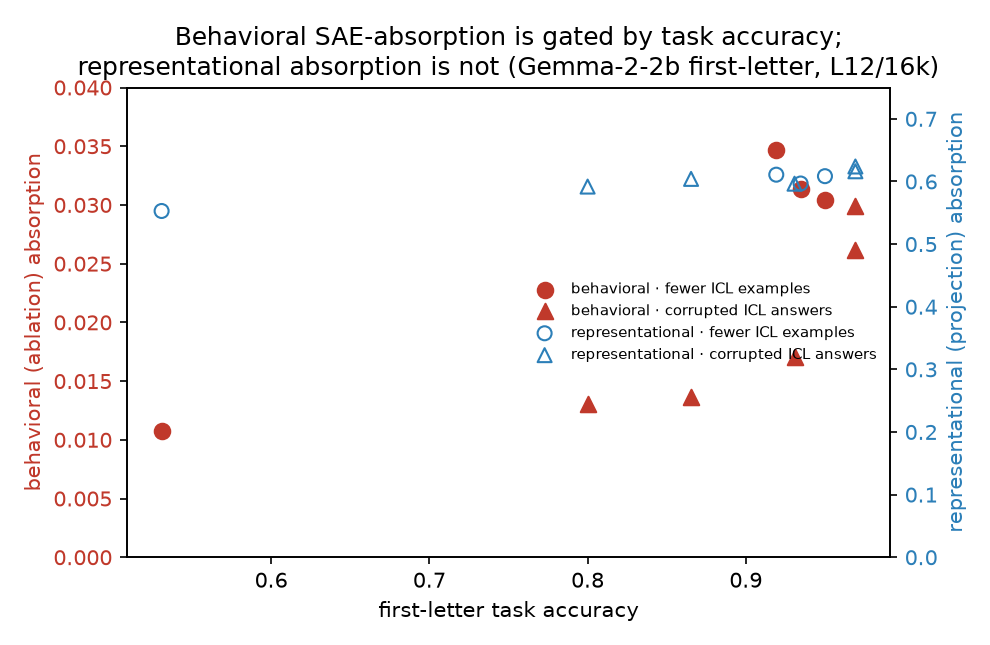
\includegraphics[width=0.62\textwidth]{figures/mechanism.png}
  \caption{Within first-letter, behavioral (ablation) absorption (red) rises with task accuracy under two
  independent manipulations, while representational (projection) absorption (blue) is flat.}
  \label{fig:mech}
\end{figure}

\section{Discussion}
The defensible reading is a \emph{metric-validity} one. For a distributed structural feature (\iscap{}),
the SAEBench-standard projection metric's ``single dominant latent'' criterion reads modestly above chance,
yet there is no causal single-latent correlate: ablation, in a regime where it works for spelling and where
the model performs the task, reports a clean zero. In other words, the projection metric appears to
\emph{over-report} single-latent absorption for a feature whose concept direction is carried by the
residual but not concentrated in one causally-load-bearing latent.

We cannot fully rule out the most natural alternative, and we state it plainly: \emph{feature hedging}
\citep{chanin2025hedging}. Capitalization is a high-frequency, broadly co-occurring concept; a $16$k SAE
may simply spread it across several latents, so that ``one dominant latent by projection geometry'' is a
weak, partly-geometric signal rather than a token-aligned absorber the model uses. Under this view our
result is best read not as a deep ``representational-vs-causal dissociation'' but as concrete evidence
that a representational absorption signal, at least for distributed features, does not imply a causal one---
consistent with the broader argument that interpretability claims need causal validation.

\section{Limitations}
Our effects are small. Spelling behavioral absorption is only ${\sim}0.01$--$0.05$ anywhere, and the
\iscap{} projection signal is marginal above its null at $n{=}130$. Only one structural property is
well-powered (\textsc{all-caps} and the suffix properties have $n{=}9$--$33$ and are anecdotal), so
``property-type-dependent'' is effectively an $n{=}1$ claim. Both models are from one family (Gemma-2,
cross-\emph{scale} only) and we use a single SAE recipe (JumpReLU/Gemma Scope); we run no non-JumpReLU or
Matryoshka SAE. Finally, we show no downstream task in which trusting the projection-flagged absorption
would demonstrably mislead---the ``so what'' that would elevate a caveat into an actionable finding.

\section{Conclusion}
Measuring SAE feature absorption off the spelling task exposes a disagreement between its two standard
metrics: for \iscap{}, the projection metric reports weak-but-above-null absorption that the ablation
metric denies, and controls show the denial is neither a task-performance nor a layer artifact. The most
likely mechanism is feature hedging, and the honest headline is a metric-validity caveat: representational
absorption signals for distributed structural features can lack a causal correlate. The natural next steps
that would turn this from a single marginal case into a robust, transferable claim are to establish the
disagreement on a second SAE architecture (e.g.\ TopK or Matryoshka) and a second, well-powered structural
property, and to exhibit a downstream decision that the mis-measurement would flip.

\paragraph{Reproducibility.}
All code, figures, and per-run numbers behind every claim above are available in the accompanying
repository, including the model-agnostic loaders used for the cross-model controls and the
independently review-verified single-class absorption pipeline.

\small
\bibliographystyle{plainnat}
\bibliography{references}

\end{document}
